\section{Torque Sensor}
The purpose of the Torque Sensor is to measure the mechanical power which is given to the sensor in the form of rotational energy from the Roll. The sensor must be able to measure both torque $\tau$ and angular velocity $\omega$ as the power P is given by:
\begin{equation}
	P=\omega\cdot\tau
\end{equation}

\subsection{Design}
The torque sensor picked by the customer is a DR-2212 Contactless Torque Sensor from Lorenz Messtechnik GmbH.

\subsection{Implementation}
Text

\begin{figure}[H]
	\centering
	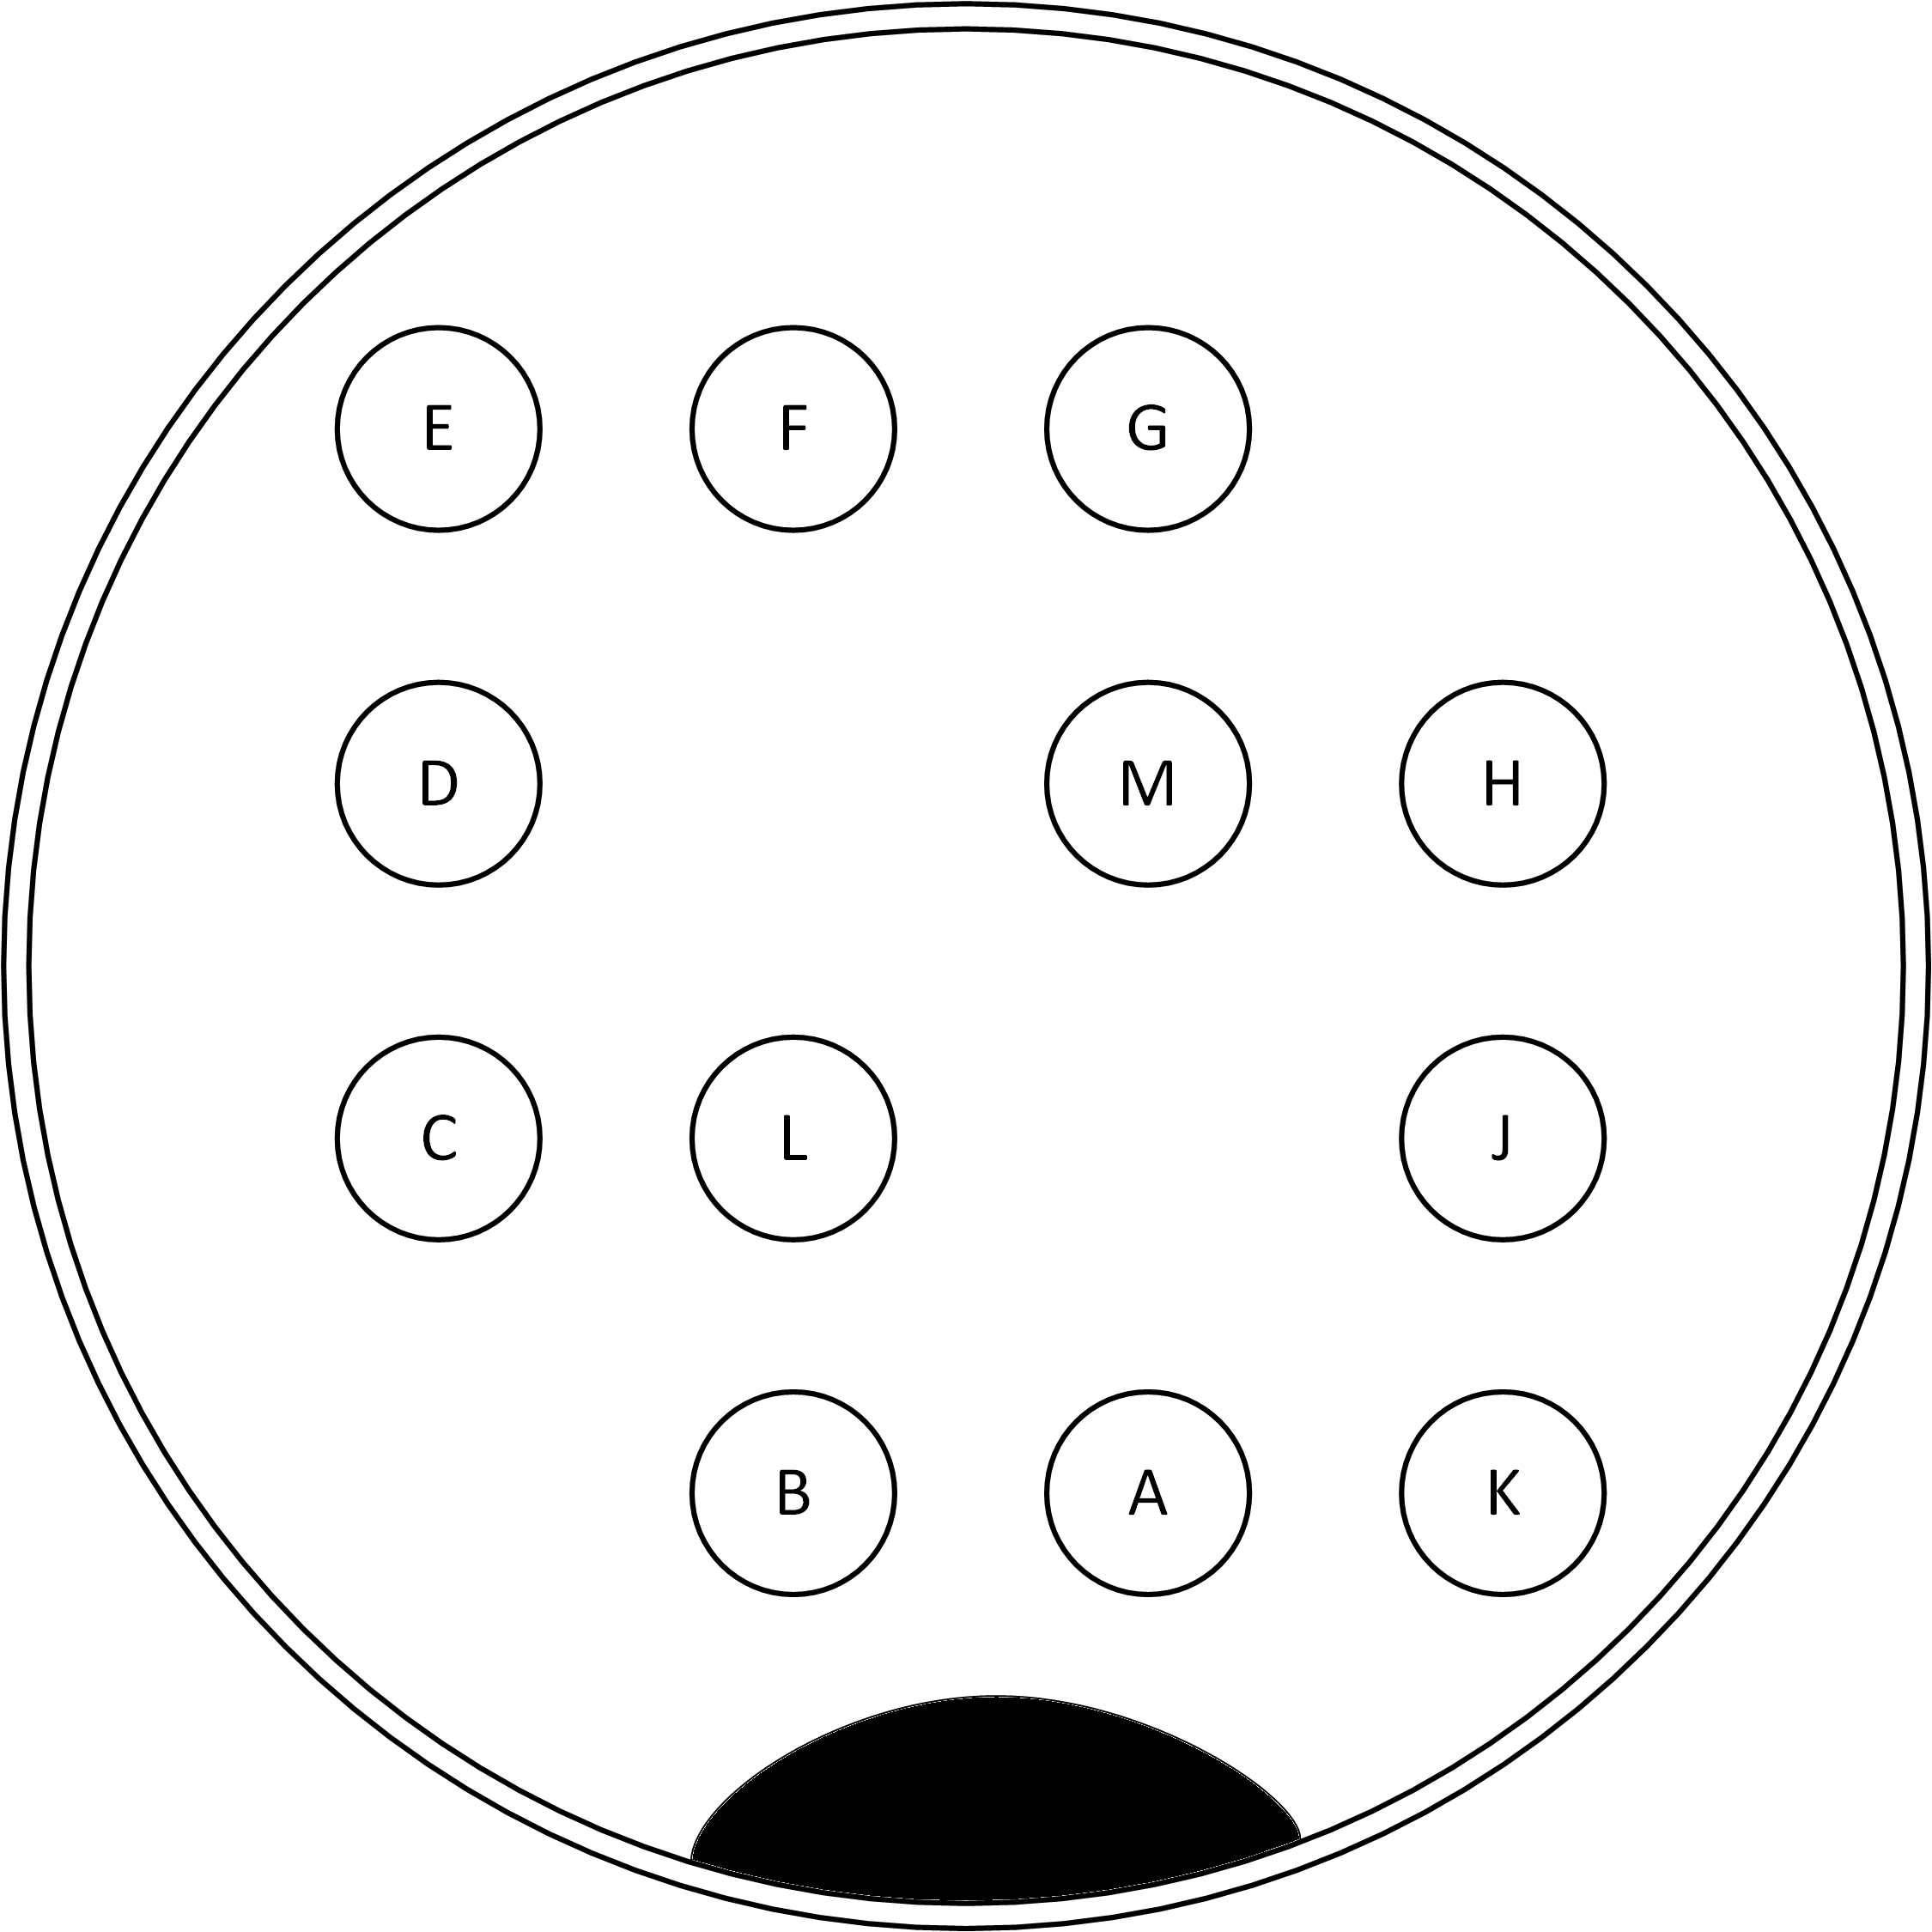
\includegraphics[width=0.3\linewidth]{Hardware/Pictures/Torque_Sensor_Pins}
	\caption{Torque Sensor Pins}
	\label{fig:Torque_pins}
\end{figure}

\subsection{Unity test}
Text